\documentclass[a4paper,12pt]{article}
\usepackage[utf8x]{inputenc}
\usepackage[swedish]{babel}
\usepackage[T1]{fontenc}
\usepackage{graphicx}
\usepackage{subcaption}
\usepackage{placeins}
\usepackage{hyperref}
\usepackage{amsfonts, amsmath, amssymb}
\usepackage{ccfonts,euler}
\usepackage{wrapfig}
\usepackage{multirow}
\usepackage{caption}
\usepackage{enumerate}
\usepackage{comment}
\usepackage[includeheadfoot,margin=1.1in]{geometry}

\usepackage{listings}
\usepackage{color}

\definecolor{dkgreen}{rgb}{0,0.6,0}
\definecolor{gray}{rgb}{0.5,0.5,0.5}
\definecolor{mauve}{rgb}{0.58,0,0.82}

\lstset{frame=tb,
  language=Python,
  aboveskip=3mm,
  belowskip=3mm,
  showstringspaces=false,
  columns=flexible,
  basicstyle={\small\ttfamily},
  numbers=none,
  numberstyle=\tiny\color{gray},
  keywordstyle=\color{blue},
  commentstyle=\color{dkgreen},
  stringstyle=\color{mauve},
  escapeinside={\%*}{*)},
  breaklines=true,
  breakatwhitespace=true,
  tabsize=3,
  literate={å}{{\r a}}1 {ö}{{\"o}}1 {ä}{{\"a}}1 {Å}{{\r A}}1 {Ö}{{\"O}}1 {Ä}{{\"A}}1
}

\oddsidemargin -15mm
\evensidemargin -15mm
\marginparwidth 5mm
\topmargin -28mm
\textheight 282mm
\textwidth 190mm
\headheight 4mm
\headsep 4mm

\sloppy

\newcounter{iii}\setcounter{iii}{0}
\def\i{\bigskip\noindent\refstepcounter{iii}\textbf{\arabic{iii}.} }
%\def\iotst#1{\par \smallskip \mbox{}\refstepcounter{iii}\hspace*{#1}\textbf{\arabic{iii}.}}
\newcounter{pun}[iii]
\def\pu{\refstepcounter{pun}{\bf(\alph{pun})}\ }
\def\Pu{\par\noindent\mbox{}\refstepcounter{pun}{\phantom{\textbf{\arabic{iii}.}}\hspace{0.2mm}\bf(\alph{pun})}\ }

\def\ext{\subsection*{Extrauppgifter}}

\title{Programmering, Pepper - Pass 4}
\date{31 juli}

\makeatletter
\let\newtitle\@title
\let\newdate\@date
\makeatother
\begin{document}

  \renewcommand*\rmdefault{ppl}\normalfont\upshape
\pagestyle{empty}
\large
\section*{\newdate\ \  \newtitle}


\i Skapa en valfri hemsida, den kan handla om dig själv, mattekollo, ditt favoritsportlag, ditt husdjur eller vad som helst. Använd gärna länkar, bilder och rubriker. 

\i Försök efterlikna sidan som är i figur~\ref{fig:boxar} så noga som möjligt. Med både CSS och HTML. 

\begin{figure}[!ht]
\centering
\includegraphics[width=0.5\textwidth]{efterlikna}
\caption{Boxar}
\label{fig:boxar}
\end{figure}


\i Skapa en knapp som man ''inte'' ska trycka på och en annan knapp som man ska trycka på. Om man trycker på fel knapp ska flera pop-up rutor komma fram, med innehåll i stil med: 
''Jag sa tryck INTE här, lär dig att lyssna...'', ''Jag varnade dig... Tryck inte på OK den här gången, så går det bättre. För de som är döva (blinda) tar jag det igen. TRYCK INTE PÅ OK'', ''OK, detta är det sista meddelandet.'', ''HA! HA! HA! HA! HA! Känn dig blåst, det var inte det sista...''

Trycker man på rätt knapp kan det också komma upp rutor: 
''Tack för att du tryckte här...''


\i

\pu Gör en funktion som heter kalleanka. För att denna funktion ska anropas ska man trycka på en länk i sidan där det står radera din hårddisk...

\pu När funktionen körs ska det komma upp en fråga som frågar om man vill radera hårddisken (vill du radera din hårddisk?). Alternativen är OK och Cancel

\pu Trycker man på OK så ska webbläsaren fråga vilken drive man vill radera (vilken drive vill du radera?). Besökaren ska få fylla i ett fält vilken drive han vill radera, drive C ska vara det som först ska vara ifyllt.

\pu Vad man än trycker på så ska en ruta säga att det inte går att radera sin hårddisken (du kan inte radera din hårddisk.).

\pu Skulle man i början trycka på Cancel så ska en ruta säga att det inte går att radera sin hårddisken (du kan inte radera din hårddisk.) (precis som förut alltså).

\i Skapa en inloggningsruta med lösenord som visar dig en hemlig del av sidan. Kanske genom att länka dig till en dold sida, eller genom att visa en pop-up med hemligt information

\i Gör en norsk miniräknare. Om man till exempel skriver in enkla tal som 0+0, 1+1 eller 0*0 så ska den lagga ihop och få problem. Testa till exempel den jag la upp på \url{www.technox.se/norsk.html}

\i Gör ett spel där man ska gissa talet mellan 0 och 100. Det skrivs ut i en textarea vad du nyss gissar, huruvida det var för stort eller för litet, och totalt antal gissningar. Förslagsvis skrivs gissningen in i ett <input type=''number'' /> fält. 

\i Låt sidan visa en random katt, genom att använda Math.random();
Katter kan ni t.ex. ladda ned här: \url{www.technox.se/katter.zip}
Kanske ha en sida som visar "Dagens katt", alltså har en specifik bild för varje veckodag. 

\ext

\i Ladda ned filerna från denna sida \url{www.technox.se/mattekollo_webb1.zip}. Skapa CSS filen och försök att styla sidan för att bli så lik figur~\ref{fig:efterlikna} som möjligt. Du får inte ändra något i HTML filen. 

\begin{figure}[!ht]
\centering
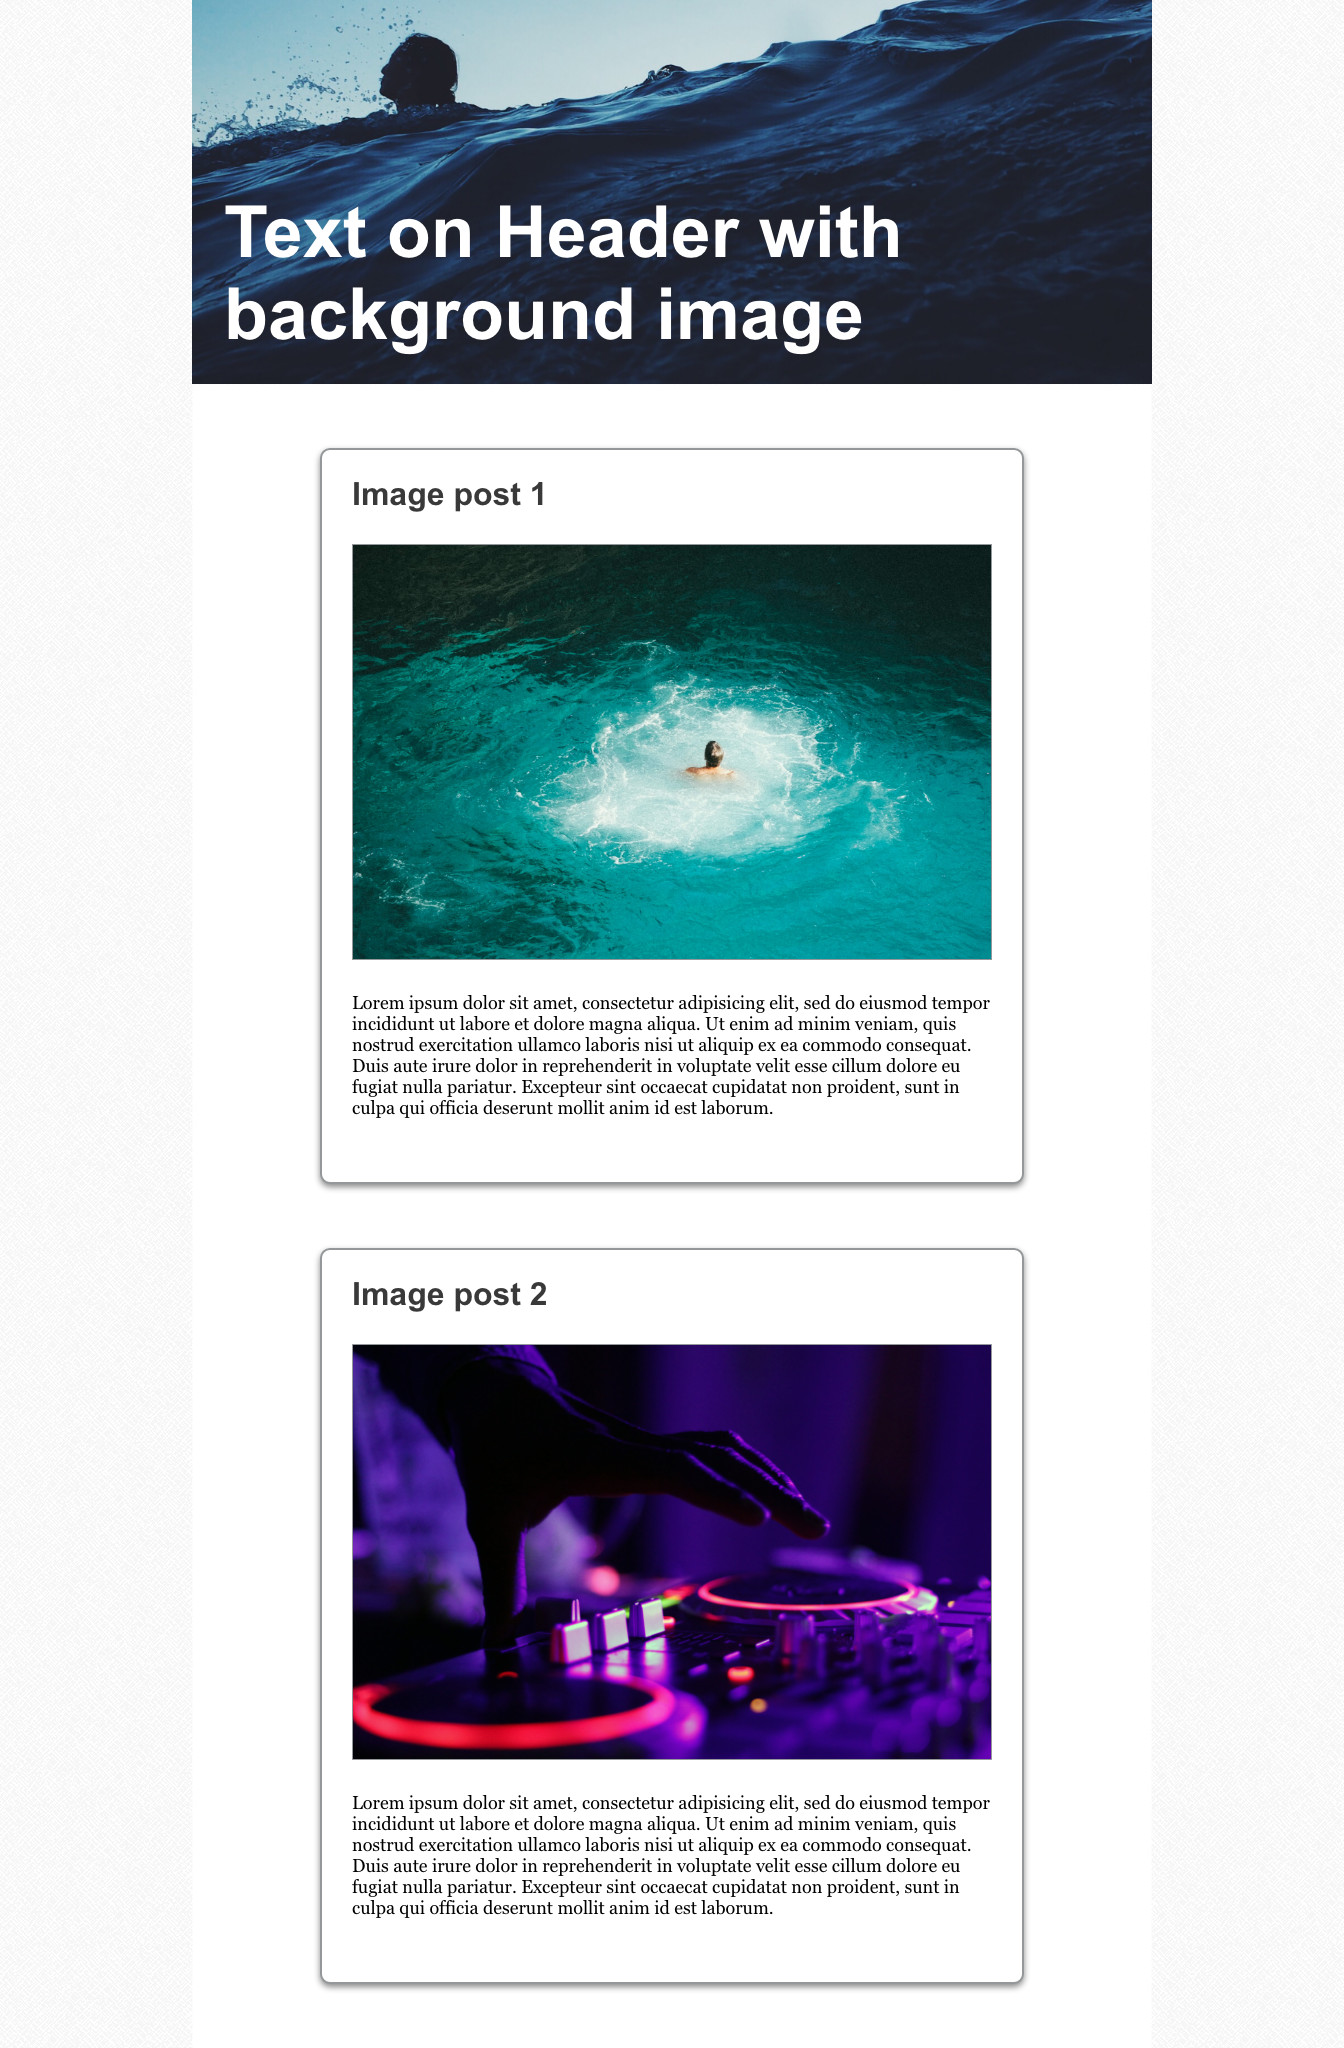
\includegraphics[width=0.5\textwidth]{efterlikna2}
\caption{En exempelsida}
\label{fig:efterlikna}
\end{figure}

\newpage 

\i Välj en sida på nätet och försök härma den. Några förslag:

\pu \url{www.finafisken.se}
\pu \url{www.marabou.se}
\pu \url{www.vaxtia.se}
\pu \url{www.likeaswede.se}

\i Du ska nu skapa ett bildspel för katter. Du kan använda bilderna i denna zip-fil om du inte vill googla fram egna katter. \url{www.technox.se/katter.zip}

\pu Skapa en hemsida (HTML och CSS) som ser ut som figur~\ref{fig:bildspel}. 

\begin{figure}[!ht]
    \centering
    \begin{subfigure}[b]{0.3\textwidth}
        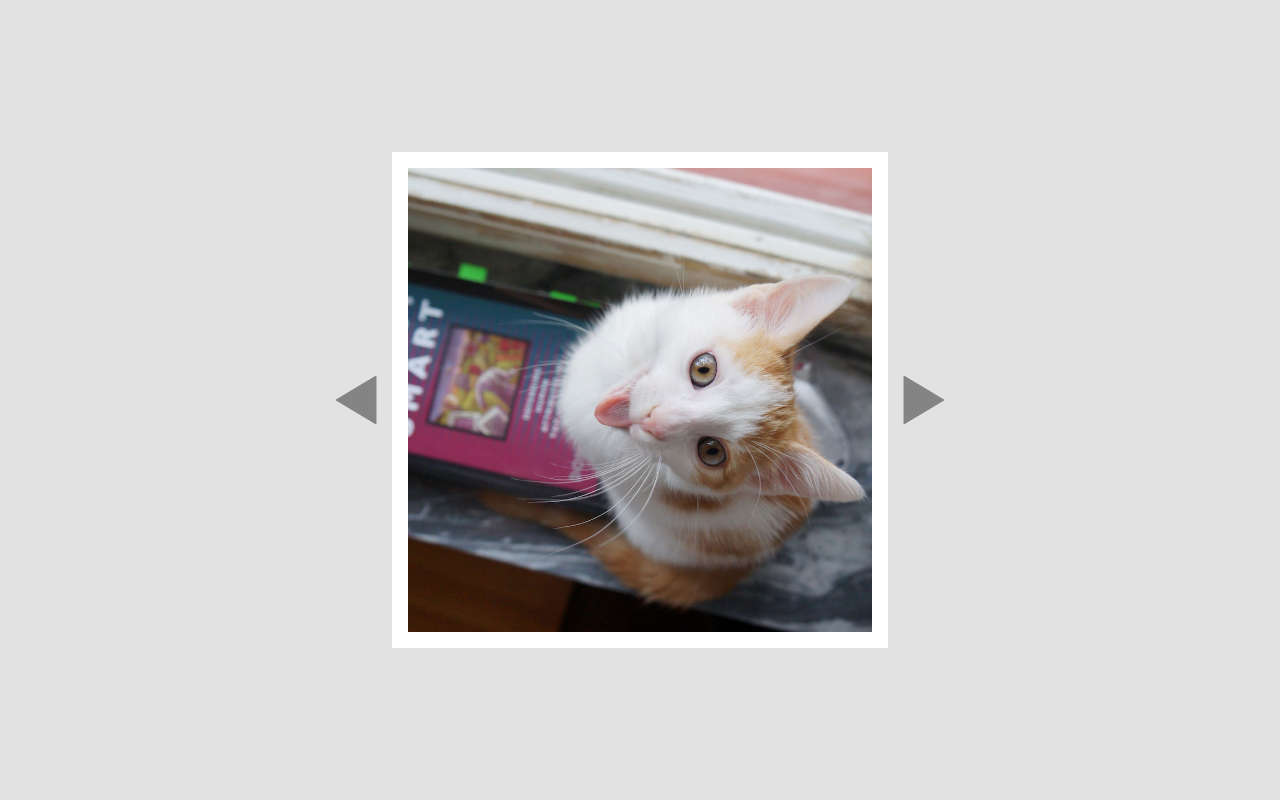
\includegraphics[width=\textwidth]{basic}
        \caption{Bildspel}
        \label{fig:bildspel}
    \end{subfigure}
    ~ %add desired spacing between images, e. g. ~, \quad, \qquad, \hfill etc. 
      %(or a blank line to force the subfigure onto a new line)
    \begin{subfigure}[b]{0.3\textwidth}
        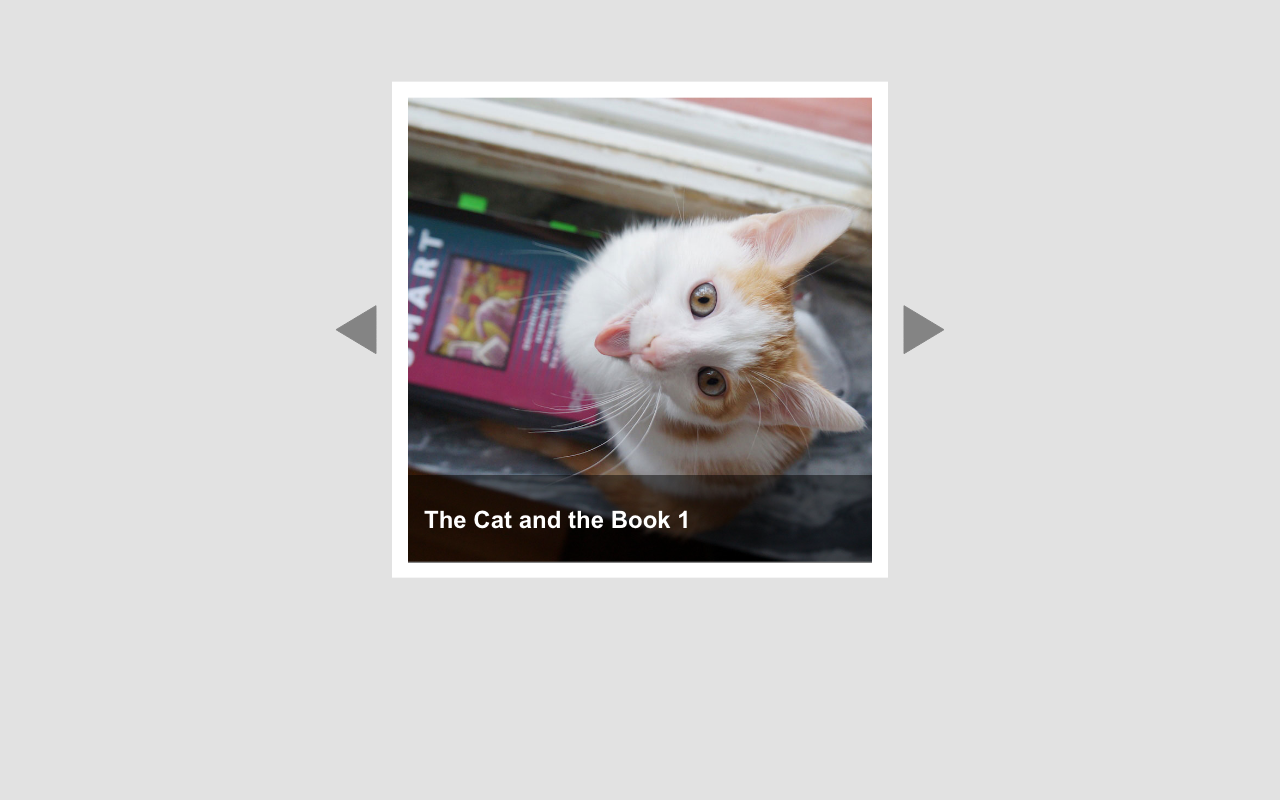
\includegraphics[width=\textwidth]{beskrivningar}
        \caption{Beskrivningar}
        \label{fig:beskrivningar}
    \end{subfigure}
    ~ %add desired spacing between images, e. g. ~, \quad, \qquad, \hfill etc. 
    %(or a blank line to force the subfigure onto a new line)
    \begin{subfigure}[b]{0.3\textwidth}
        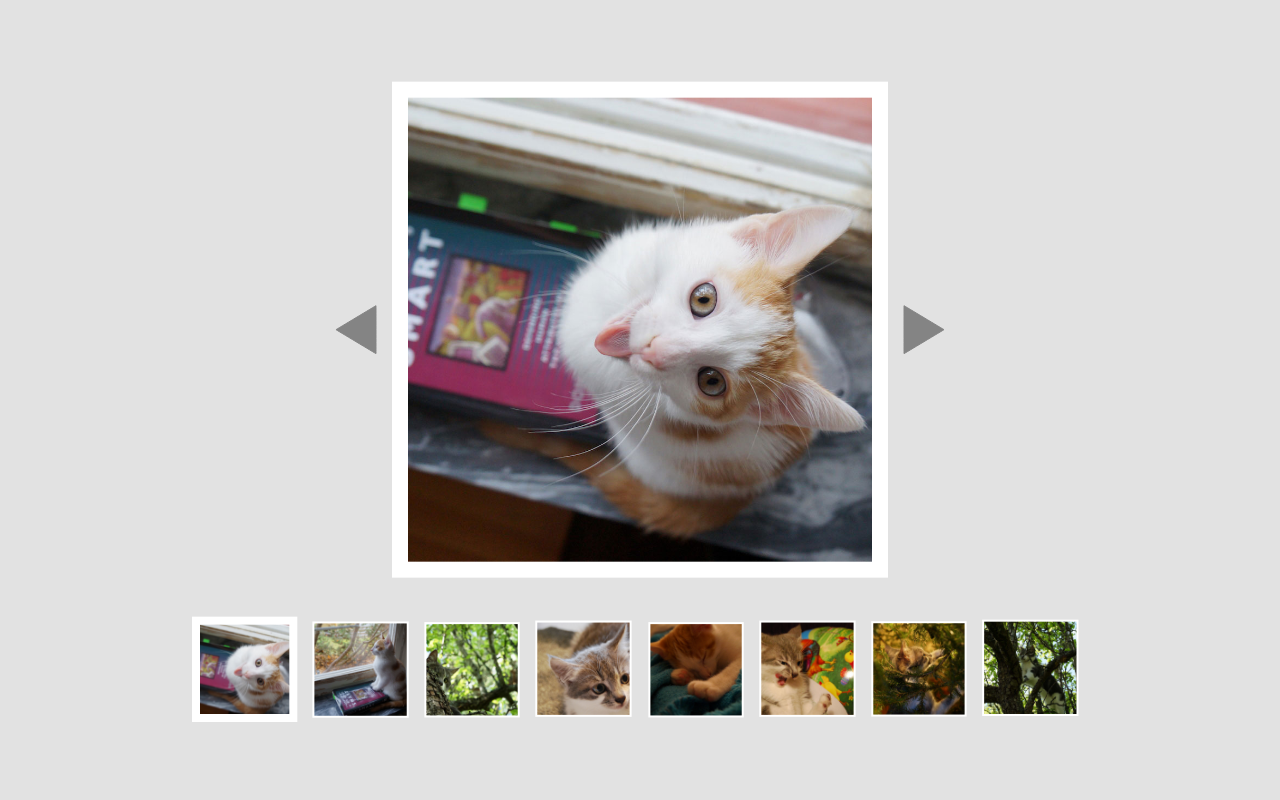
\includegraphics[width=\textwidth]{tumnaglar}
        \caption{Tumnaglar}
        \label{fig:tumnaglar}
    \end{subfigure}
    \caption{Bildspel}%\label{fig:b}
\end{figure}




%Nu ska du göra bildspelet interaktivt. Implementera följande med hjälp av JavaScript, HTML och CSS: 

\pu 
Skapa trianglar till höger och vänster om bilden som reagerar när användaren för musen över dem. Du kan till exempel ändra genomskinlighet, färg, storlek etc. 

\pu Ändra formen av muspekaren till en hand, detta hjälper användaren att förstå att hen kan klicka på triangeln. 

\pu Ändra bilden som syns i mittenrutan när användaren klickar på trianglarna. Bildspelet ska loopa, dvs när användaren klickar på "show next image" och den sista bilden visas så ska bildspelet börja om med att visa den första bilden igen. 

\pu Försök att göra koden enkel att modifiera så att fler (eller färre) bilder kan läggas till enkelt. Använd till exempel en array/lista för bilderna. 

\pu Lägg till bildbeskrivningar på bilderna i en semitransparent box över bilden. Se figur~\ref{fig:beskrivningar}


\pu Gör så att beskrivningen bara syns när man hovrar över bilden. 

\pu Lägg till tumnaglar för alla bilder i bildspelet under den större bilden. Du ska markera den bild som visas just nu, genom att till exempel lägga till en vit ram runt den, eller någon annan markör. Se figur~\ref{fig:tumnaglar}. Använd mindre bilder (färre bytes) som tumnaglar så att sidan laddas snabbare (finns i zip-filen med katter). 




\end{document}